%% LyX 2.0.8.1 created this file.  For more info, see http://www.lyx.org/.
%% Do not edit unless you really know what you are doing.
\documentclass[english]{article}
\usepackage[T1]{fontenc}
\usepackage[latin9]{inputenc}
\usepackage{listings}
\lstset{basicstyle={\scriptsize}}
\usepackage{verbatim}
\usepackage{float}
\usepackage{url}
\usepackage{graphicx}

\makeatletter

%%%%%%%%%%%%%%%%%%%%%%%%%%%%%% LyX specific LaTeX commands.
%% Because html converters don't know tabularnewline
\providecommand{\tabularnewline}{\\}
%% A simple dot to overcome graphicx limitations
\newcommand{\lyxdot}{.}

\floatstyle{ruled}
\newfloat{algorithm}{tbp}{loa}
\providecommand{\algorithmname}{Algorithm}
\floatname{algorithm}{\protect\algorithmname}

%%%%%%%%%%%%%%%%%%%%%%%%%%%%%% User specified LaTeX commands.
\usepackage{tikz}
\usepackage{tkz-graph}
\usepackage{pgf}
\usetikzlibrary{arrows,automata}

\makeatother

\usepackage{babel}
\begin{document}

\title{Should protracted speciation be incorporated in phylogenetic tree
construction methods?}


\author{Rich�l J.C. Bilderbeek \& Rampal S. Etienne}

\maketitle

\section{Abstract}

The construction of phylogenies has proven invaluable in answering
evolutionary biological questions. Our current phylogenetic tools
ignore the fact that speciation takes time, which may have a profound
effect in phylogeny reconstruction. Here, we measure the errors our
current tools give when recovering simulated phylogenies, for different
speciation durations. It has been found that branch lengths are consistently
and strongly underestimated for biologically relevant parameters.
This research shows that protractedness is a complexity of nature
that should not be ignored and should be incorporated in our phylogenetic
tools.


\section{Introduction}


\paragraph{Speciation takes time}

Although we know that speciation takes time, we commonly ignore this
when constructing a phylogeny, by chosing a constant-rate birth-death
model as a speciation model. The constant-rate birth-death model (as
described in for example \cite{nee1994}) is among the simplest speciation
models, and assumes instant speciation and extinction rates, captured
by its two parameters. The constant-rate birth-death model is popular
for its simplicity, yet has also served as a starting point for more
elaborate specation models.


\paragraph{Other non-protracted speciation models}

Other speciation models may assume that speciation rate changes in
time {[}REF{]}, is dependent on the amount of species present \cite{etienne2011diversity},
or is trait dependent {[}REF{]}. The original model by making speciation
rate dependent on time, diversity or trait value. Also these extended
models assume speciation is instantaneous.


\paragraph{Protracted speciation model}

There is, however, a speciation model family that does assume speciation
takes time: the protracted speciation model family \cite{etienne2012prolonging},
which extends the constant-rate birth-death model by adding an additional
species state (see also figure \ref{fig:The-states-and-transitions-of-a-species}).
It is called a model family, as it makes no assumption about speciation
and extinction rates: these may be contant or depend on time, diversity
or trait value.


\paragraph{Use of a speciation model in inferring a phylogeny}

Speciation models do not exist for theoretical purposes only, but
are widely used to make inferences from genetic data. There are multiple
computer programs to create phylogenies and/or parameter estimates
from aligned DNA sequences. One such tool is BEAST2 \cite{bouckaert2014beast},
which allow for a Bayesian approach to phylogenetics. BEAST2 supplies
the user with multiple speciation models, yet all assume instantaneous
speciation. 


\paragraph{This study}

This simulation investigates the consequence of BEAST2 using instantaneous
speciation, by creating a 'true' tree that is protracted and seeing
how well BEAST2 can recover it. It is expected that for higher protractedness
(thus deviation from BEAST2 its assumptions), the error will increase.
It is unknown, however, if and when this error is relevant. 


\paragraph{Preview results}

This study shows that {[}TODO: put result here{]}


\section{Methods}


\subsection{Model}

The speciation model used in this investigation is a constant-rate
protracted speciation model.

A protracted speciation model assumes that species have at least two
states: a species is either a good or incipient species. A good species
is a species recognized as such, where an incipient species is not
yet. Both good and incipient species can generate new incipient species,
at the speciation-initiation rates $b_{g}$ and $b_{i}$ respectively.
An incipient species can become a good species at the speciation-completion
rate $\lambda$. Both good and incipient species can go extinct at
rates $\mu_{i}$ and $\mu_{g}$ respectively (see also figure \ref{fig:The-states-and-transitions-of-a-species}).

The simplest member of the protracted speciation famility is the constant-rate
protracted speciation model, which assumes that all rates are constant
in time.

\begin{figure}[H]
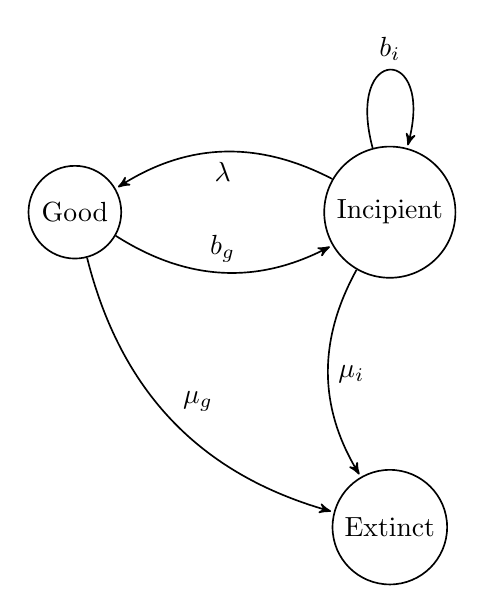
\begin{tikzpicture}[->,>=stealth',shorten >=1pt,auto,node distance=4cm, semithick]   
\tikzstyle{every state}=[]
\node[state] (A)              {Good};   
\node[state] (B) [right of=A] {Incipient};   
\node[state] (C) [below of=B] {Extinct};   
\path (A) edge [bend right] node {$b_g$} (B)
      (A) edge [bend right] node {$\mu_g$} (C)
      (B) edge [loop above] node {$b_i$} (B)
      (B) edge [bend right] node {$\lambda$} (A)
      (B) edge [bend right] node {$\mu_i$} (C); 
\end{tikzpicture}

\caption{The states and transitions of a species. $b_{i}$: speciation-initiation
rate of incipient species. $b_{g}$: speciation-initiation rate of
good species. $\lambda$: speciation completion rate. $\mu_{i}$:
extinction rate of incipient species. $\mu_{g}$: extinction rate
of good species. Figure after Etienne et al, 2014, Evolution\label{fig:The-states-and-transitions-of-a-species}}
\end{figure}


There is no relationship known between the speciation rate (often
called $\lambda$) of the constant-rate birth-death model and a combination
of the speciation-initiation $\lambda$ and speciation-completion
rates of the protracted birth-death model ($b_{g}$ and $b_{i}$).
When setting $\lambda\rightarrow\infty$, the model used falls back
to a constant-rate (non-protracted) birth-death model.


\subsection{Workflow}


\subsubsection{Creating gene trees}

From a parameter combination, a 'true' protracted constant-rate birth-death
gene tree is simulated in the R programming language \cite{R}, using
the PBD package \cite{PBD}.


\paragraph{Speciation-completion rate}

The speciation-completion rate $\lambda$ is pivotal for this study,
as when $\lambda\rightarrow\infty$ the model falls back to a birth-death
model and satisfies the instantaneous speciation assumption of the
tools used.


\paragraph{Speciation initiation rate, extinction rate and crown age}

The parameter values for the speciation-initiation rates $b$, extinction
rate $\mu$ and phylogeny crown age $t_{c}$ need to be balanced,
as $t_{c}b\gg\mu$ results in overly taxa-rich phylogenies, where
$t_{c}\mu\gg b$ results in excessively frequent extinctions. As a
starting point, we used the parameters used by \cite{etienne2014estimating}.
For simplicity, we assume species can give rise to new species, independent
of species status, thus $b_{i}=b_{g}$ {[}TODO: Is there reason to
assume differently?{]}. Additionally, we assume a species can go extinct
independent of species status, so$\mu_{i}=\mu_{g}$ {[}TODO: Is there
reason to assume differently?{]}. 


\subsubsection{Creating species trees}

The longer speciation takes, the higher the number of incipient species
will be. Because BEAST2 assumes one individual per species, we randomly
sample one individual per species of all species to obtain a species
tree. This is replicated $n_{s}$ times. Also an outgroup is added,
so that the phylogeny inferring software can root a phylogeny. 


\subsubsection{Creating a DNA alignment}

From each species tree, $n_{a}$ DNA alignments were simulated following
a Jukes-Cantor nucleotide subsititution model using the phangorn R
package \cite{phangorn}.

In creating DNA sequence alignments from the phylognies, a mutation
rate $r$ and DNA sequence length $l_{a}$ need to be balanced as
well. As a starting point, we chose the DNA sequence length to be
1kb, as this a common gene sequence length, but we also included one
and two orders of magnitude bigger. The mutation rate is chosen to
match a mutation rate as in nature {[}TODO: find that value{]}.


\subsubsection{Creating a BEAST2 posterior}

From these DNA alignments, a posterior containing phylogenies and
parameter combinations were constructed using the BEAST2 software
package \cite{bouckaert2014beast}. Per alignment, $n_{b}$ BEAST2
runs were performed, each with an MCMC length of $l_{m}$, to see
if both runs result in similar posteriors. 

The BEAST2 priors used were as follows: 

For the site model, the default parameters were used: which is the
Jukes-Cantor substitution model.

For the clock model, the default parameters are used, which is a strict
clock prior, with a clock rate of $1.0$.

For the tree prior, the 'Birth Death Model' was selected and its parameters
kept at the default uniform birth-rate  (range $0$-$10^{5}$, initial
value $1$) and default uniform birth-rate  (range $0$-$1$, initial
value $0.5$).


\subsubsection{All parameters used}

Table \ref{tab:Parameters-used} shows all parameter values used.

\begin{table}
\begin{tabular}{|c|c|}
\hline 
Parameters & Values\tabularnewline
\hline 
\hline 
$b=b_{g}=b_{i}$ & $0.1$, $0.2$, $0.4$, $0.8$\tabularnewline
\hline 
$\lambda$ & $0.0$, $0.1$, $0.2$, $0.4$, $0.8$, $10^{6}$\tabularnewline
\hline 
$\mu=\mu_{g}=\mu_{i}$ & $0.0$, $0.1$, $0.2$, $0.4$, $0.8$\tabularnewline
\hline 
$t_{c}$ & $15$\tabularnewline
\hline 
$r$ & $10^{-1}$,$10^{-2}$,$10^{-3}$\tabularnewline
\hline 
$l_{a}$ & $10^{3}$,$10^{4}$,$10^{5}$\tabularnewline
\hline 
$n_{s}$ & $2$\tabularnewline
\hline 
$n_{a}$ & $2$\tabularnewline
\hline 
$n_{b}$ & $2$\tabularnewline
\hline 
$l_{m}$ & $10^{6}$\tabularnewline
\hline 
\end{tabular}

\caption{Parameters used\label{tab:Parameters-used}}
\end{table}



\subsection{Analyzing the results}

These posteriors were analyzed using bash (\url{www.gnu.org/software/bash})
scripts and the R programming language \cite{R}, using the packages
rBEAST \cite{rBEAST} to process BEAST2 output files, ape \cite{APE}
and ggplot2 \cite{ggplot2} for plotting and testit \cite{testit}
for debugging. All the scripts can be downloaded \url{https://github.com/richelbilderbeek/should}. 


\section{Results}


\section{Discussion }

A constant-rate protracted birth-death model is used, this research
could easily be modified to compare other protracted birth-death models,
for example, a diversity-dependent protracted birth-death model. There
has been now work done on the diversity-dependent protracted birth-deatg
model yet.

This research assumes that speciation is allopatric, because in the
simulation of the DNA alignments, there is no gene flow anymore between
two taxa of still-the-same species. 

\bibliographystyle{plain}
\bibliography{ShouldProtractedSpeciationBeIncorporatedInPhylogeneticTreeConstructionMethods}


\appendix

\section{Worked-out examples\label{sec:Worked-out-examples}}

To better understand the steps performed in this research, I show
here some worked-out examples in detail. 


\subsection{Workflow\label{sub:Workflow}}

Every experiment has the following steps:
\begin{itemize}
\item Creating parameter files: see chapter \ref{sub:Creating-parameter-files}
\item Checking your parameter file: see chapter \ref{sub:Checking-your-parameter-file}
\item Do simulations: see chapter \ref{sub:Do-simulations}
\item Analyze results: see chapter \ref{sub:Analyze-results}
\end{itemize}
Figure \ref{fig:Workflow} shows the workflow graphically:

\begin{figure}[H]
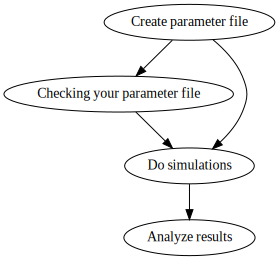
\includegraphics[scale=0.75]{Workflow_experiment}

\caption{The chronological order of the experiment\label{fig:Workflow}}
\end{figure}


Each step can be done from a command-line script, so that a computer
cluster can conveniently work on it.


\subsubsection{Creating parameter files\label{sub:Creating-parameter-files}}

Parameter files can be created from the command line by supplying
all the arguments to the script 'create\_parameter\_file.R' (see chapter
\ref{sub:create_parameter_file.R}). 


\subsubsection{Checking your parameter file\label{sub:Checking-your-parameter-file}}

You can check if you created a parameter file with the correct arguments
using the R script 'check\_parameter\_file.R' (see chapter \ref{sub:check_parameter_file.R}).


\subsubsection{Do simulations\label{sub:Do-simulations}}

A simulation (including its replicates) can be run from the command
line by supplying all the arguments to the R script 'do\_simulation.R'
(see chapter \ref{sub:do_simulation.R}). This will result in:
\begin{itemize}
\item A parameter file with intermediate data added
\item BEAST2 output files
\end{itemize}

\subsubsection{Analyze results\label{sub:Analyze-results}}

After the simulations, the results are analyzed with the R script
'do\_analyze.R' (see chapter \ref{sub:do_analyze.R}).


\subsection{Experiments}

These worked-out examples show:
\begin{itemize}
\item the error if protractedness is absent: example 1, see chapter \ref{sub:Example-1-Weak-protractedness}
\item the error if protractedness strong: example 2, see chapter \ref{sub:Example-2-Strong-protractedness}
\item comparing the errors of example 1 and 2: see chapter \ref{sub:Comparing-example-1-and-2}
\item the error if protractedness is absent for multiple replicates: example
3, see chapter 
\item the error if protractedness is strong for multiple replicates: example
4, see chapter 
\item comparing the errors of example 3 and 4: see chapter 
\end{itemize}
An overview of all parameter settings can be seen in table \ref{tab:Examples-parameters},
which can be created by calling the 'create\_example\_parameter\_files.sh'
script .

\begin{table}
\begin{tabular}{|c|c|c|c|c|}
\hline 
Example & 1 & 2 & 3 & 4\tabularnewline
\hline 
\hline 
Protracted? & No & Yes & No & Yes\tabularnewline
\hline 
 RNG seed & \multicolumn{4}{c|}{1}\tabularnewline
\hline 
$b=b_{g}=b_{i}$ & \multicolumn{4}{c|}{0.5}\tabularnewline
\hline 
$\lambda$ & $10^{6}$ & $10^{-1}$ & $10^{6}$ & $10^{-1}$\tabularnewline
\hline 
$\mu=\mu_{g}=\mu_{i}$ & \multicolumn{4}{c|}{0.1}\tabularnewline
\hline 
$t_{c}$ & \multicolumn{4}{c|}{5}\tabularnewline
\hline 
$t_{s}$ & \multicolumn{2}{c|}{1} & \multicolumn{2}{c|}{4}\tabularnewline
\hline 
$r$ & \multicolumn{4}{c|}{0.01}\tabularnewline
\hline 
$n_{a}$ & \multicolumn{2}{c|}{1} & \multicolumn{2}{c|}{4}\tabularnewline
\hline 
$l_{a}$ & \multicolumn{4}{c|}{1000}\tabularnewline
\hline 
$n_{b}$ & \multicolumn{2}{c|}{1} & \multicolumn{2}{c|}{4}\tabularnewline
\hline 
$l_{m}$ & \multicolumn{4}{c|}{$10^{6}$}\tabularnewline
\hline 
\end{tabular}

\caption{Parameters used in the examples\label{tab:Examples-parameters}}


\end{table}


The parameter settings used in this example are identical, except
for their speciation completion rate and number of replicates. 

Creating these parameter files is shown in chapter \ref{sub:Creating-parameter-files}.

The experimental setup of this research has multiple steps, which
we will follow closely here. These steps are described in chapter
\ref{sub:Workflow}.

These worked-out examples show the data produced in its raw form and
does not care too much about aesthetics.


\subsection{Example 1: Weak protractedness\label{sub:Example-1-Weak-protractedness}}

This example answers the question: what is the base level error of
the analyses in this research?

The base level error can be obtained by using parameters for a constant-rate
birth-death model. All tools used assume this model, but there will
be noise (thus error) added in the process. 

The parameter settings of example 1 have a high speciation completion
rate $\lambda$, which makes the constant-rate protracted speciation
model fall back to a constant-rate birth-death model, as incipient
species become good species (close to) instantaneously.


\subsubsection{Gene tree}

The first step is to simulate a gene tree. For our parameters, this
results in the tree in figure \ref{fig:Example-1-gene-tree}

\begin{figure}[H]
\includegraphics[width=0.5\textwidth]{/home/p230198/GitHubs/R/Peregrine/example_1_gene_tree}

\caption{Example 1 gene tree. The taxon labels are S{[}genus{]}-{[}species{]}-{[}sub-species{]}'.
This plot is created by the function 'plot\_gene\_tree'\label{fig:Example-1-gene-tree}}


\end{figure}



\subsubsection{Species tree}

From that gene tree, we create a species tree by sampling one individual
per species. Because speciation is instantenous for a constant-rate
birth death model, there exist no multiple individuals per species.
To being able to root our phylogenies in later steps, an outgroup
is added as well, resulting in figure \ref{fig:Example-1-species-tree}:

\begin{figure}[H]
\includegraphics[width=0.5\textwidth]{/home/p230198/GitHubs/R/Peregrine/example_1_species_tree_with_outgroup_1}

\caption{Example 1 species tree. This plot is created by the function 'plot\_species\_tree\_with\_outgroup'\label{fig:Example-1-species-tree}}
\end{figure}


\begin{figure}[H]
\includegraphics[width=0.5\textwidth]{/home/p230198/GitHubs/R/Peregrine/example_1_species_tree_with_outgroup_nltt_1}

\caption{Example 1 species tree its nLTT plot. This plot is created by the
function 'plot\_species\_tree\_with\_outgroup\_nltt'\label{fig:Example-1-species-tree-nltt}}
\end{figure}



\subsubsection{Alignment}

Knowing the evolutionary distances between species, DNA sequence alignments
can be simulated fitting the tree. To do so, the parameters for sequence
length and mutation rate are used. Note that this research assumes
a simple Jukes-Cantor model, and does so as well in later steps.

Figure \ref{fig:Example-1-alignment} shows a visualisation of the
simulated alignment of our example:

\begin{figure}[H]
\includegraphics[width=0.5\textwidth]{/home/p230198/GitHubs/R/Peregrine/example_1_alignment_1_1}

\caption{Example 1 alignment. This figure is created using the function 'plot\_alignments'\label{fig:Example-1-alignment}}
\end{figure}



\subsubsection{Posterior}

With BEAST2 we can now obtain a posterior. A posterior consists of
a representative sample of all possible trees (and parameter estimates),
yet with more probable trees being present more often.

After running BEAST2 on our DNA sequence, the full posterior must
be verified to be eligible for further analysis. Using Tracer, we
can open the .log file generated by BEAST2, which is then displayed
as shown in figure \ref{fig:Example-1-ess-and-trace}:

\begin{figure}[H]
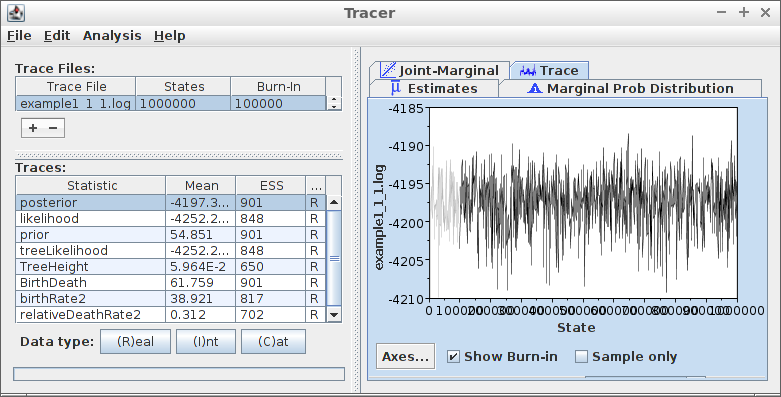
\includegraphics[width=1\textwidth]{example_1_trace}

\caption{Example 1 its ESSes and trace log\label{fig:Example-1-ess-and-trace}}
\end{figure}


It can be seen that the values for ESS (Effective Sample Size) are
above 200 and that the trace log shows a well-mixed chain. An ESS
of 200 is used as a minimum in this research. 

Now that the full posterior is assumed to be correct, I will now highlight
one state of it first, before going back to the full picture. In this
case, I choose the last state to zoom in on. I take the last state
for no specific reason and I could just as easily have picked the
first or a random one. From this last state, I take the tree only.
This last tree may be very different by chance, as unlikely trees
are present, yet in low abundances. 

The tree picked from the posterior is shown in figure \ref{fig:Example-1-posterior-sample-tree}:

\begin{figure}[H]
\includegraphics[width=0.5\textwidth]{/home/p230198/GitHubs/R/Peregrine/example_1_posterior_sample_1_1_1}

\caption{A random species tree from example 1 its posterior. This figure is
produced by the function 'plot\_posterior\_samples'\label{fig:Example-1-posterior-sample-tree}}
\end{figure}


The species tree picked from the posterior does not look too different
compared to the original species tree (figure \ref{fig:Example-1-species-tree}).
To get a better view of their resemblance, their nLTT plots are put
in the same chart in figure \ref{fig:Example-1-posterior-sample-tree-nltt}

\begin{figure}[H]
\includegraphics[width=0.5\textwidth]{/home/p230198/GitHubs/R/Peregrine/example_1_posterior_sample_nltt_1_1_1}

\caption{The nLTTs of the true species tree (solid black line) and the species
tree sampled from example 1 its posterior (dotted line). This figure
is produced by the function 'plot\_posterior\_sample\_nltts'\label{fig:Example-1-posterior-sample-tree-nltt}}
\end{figure}


We can observe that the lines are close, but do not match. Also this
is expected, due to stochasticity in the MCMC sampling.

A posterior contains many phylogenies. Before analysing them, the
tool 'densitree' can be used to view these:

\begin{figure}[H]
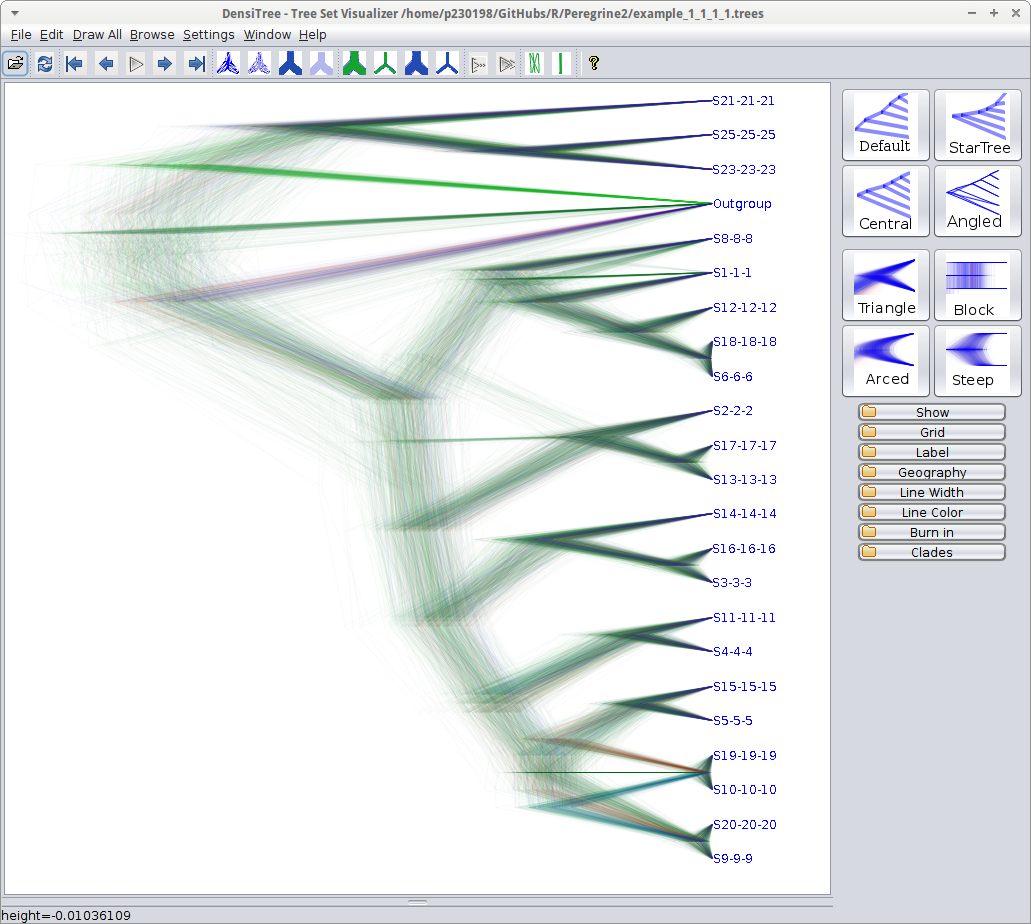
\includegraphics[width=0.5\textwidth]{example_1_densitree}

\caption{Example 1 its posterior its phylogenies\label{fig:Example-1-densitree}}
\end{figure}


To derive at a quantity of the match between true/input tree and the
posterior, one can sum the error between the true and posterior tree
nLTT plot, see {[}Janzen{]}. For this example, the error between the
true species tree and the posterior tree is $0.026$. The true species
tree can be compared to every tree in the posterior, calculating the
nLTT statistic for each. This will results in the following histogram:

\begin{figure}[H]
\includegraphics[width=0.5\textwidth]{/home/p230198/GitHubs/R/Peregrine/example_1_nltt_stats_1_1_1}

\caption{Histogram of the nLTT statistic between the true species tree and
the trees in the posterior. This figure is produced by the function
'plot\_posterior\_nltt\_stats\_histogram'\label{fig:Example-1-nltt-stats}}
\end{figure}


Here we can see that this histogram looks a bit like a Poisson or
Gamma distribution, with a median at $0.02-0.025$. 

But this does not tell us where the errors have been made: near the
crown, near the tips, or in between? To do so, we plot the average
nLTT plot of the posterior and compare it to the true species tree
its nLTT, as shown in figure \ref{fig:Example-1-posterior-average-nltt}:

\begin{figure}[H]
\includegraphics[width=0.5\textwidth]{/home/p230198/GitHubs/R/Peregrine/example_1_posterior_average_nltt_1_1_1}

\caption{Average nLTT of all the trees in the posterior. Solid line: nLTT of
true species tree. Dotted line: average nLTT of all posterior trees.
This figure is produced using the function 'plot\_posterior\_average\_nltts'\label{fig:Example-1-posterior-average-nltt}}
\end{figure}



\subsection{Example 2: Strong protractedness\label{sub:Example-2-Strong-protractedness}}

This example answers the question: how do the analyses of this research
look like for strong protractedness?

The pipeline is identical, except one parameter is changed: the speciation
completion rate $\lambda$ is set to a low value.


\subsubsection{Gene tree}

The gene tree simulated is shown in figure \ref{fig:Example-2-gene-tree}:

\begin{figure}[H]
\includegraphics[width=0.5\textwidth]{/home/p230198/GitHubs/R/Peregrine/example_2_gene_tree}

\caption{Example 2 gene tree. The taxon labels are S{[}genus{]}-{[}species{]}-{[}sub-species{]}'\label{fig:Example-2-gene-tree}}
\end{figure}


Note that there are only four complete species here, called S1-1 to
S4-4. The third label is the sub-species label. Also note that S1-1
is a polyphylic species.


\subsubsection{Species tree\label{sub:Species-tree}}

From that gene tree, we create a species tree by sampling one individual
per species. With speciation taking a long time to complete, there
are indeed many incipient species present, and only four different
full species. Random picking one individual per species, and adding
an outgroup, results in the species tree of figure \ref{fig:Example-2-species-tree}:

\begin{figure}[H]
\includegraphics[width=0.5\textwidth]{/home/p230198/GitHubs/R/Peregrine/example_2_species_tree_with_outgroup_1}\includegraphics[width=0.5\textwidth]{/home/p230198/GitHubs/R/Peregrine/example_2_species_tree_with_outgroup_nltt_1}

\caption{Example 2 species tree\label{fig:Example-2-species-tree}}
\end{figure}



\subsubsection{Alignment}

The DNA sequences are simulated over the species tree. Because there
have been only four species and one outgroup, there will be five DNA
sequences generated, as shown in figure \ref{fig:Example-2-alignment}:

\begin{figure}[H]
\includegraphics[width=0.5\textwidth]{/home/p230198/GitHubs/R/Peregrine/example_2_alignment_1_1}

\caption{Example 2 alignment\label{fig:Example-2-alignment}}
\end{figure}



\subsubsection{Posterior}

BEAST2 is again used to create a representative sample of all possible
trees (and parameter estimates) from those alignments and checked
visually by Tracer (see figure \ref{fig:Example-2-ess-and-trace}).

\begin{figure}[H]
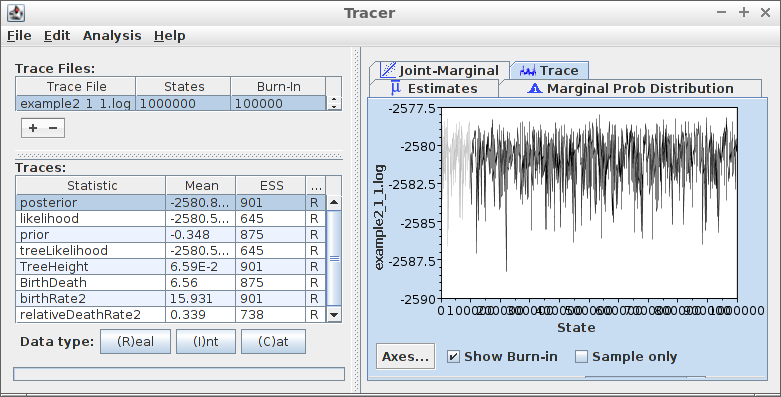
\includegraphics[width=1\textwidth]{example_2_trace}

\caption{Example 2 its ESSes and trace log\label{fig:Example-2-ess-and-trace}}
\end{figure}


Again all ESS values are above 200 and that the trace log shows a
well-mixed chain. 

Also here, we pick a random tree from the posterior (in this case,
the last one):

\begin{figure}[H]
\includegraphics[width=0.5\textwidth]{/home/p230198/GitHubs/R/Peregrine/example_2_posterior_sample_1_1_1}\includegraphics[width=0.5\textwidth]{/home/p230198/GitHubs/R/Peregrine/example_2_posterior_sample_nltt_1_1_1}

\caption{A random species tree (and its nLTT plot) from example 2 its posterior\label{fig:Example-2-posterior-sample-tree}}
\end{figure}


We expect this tree from the posterior to match the true species tree
less well, as all the tools used assume instant speciation, where
we simulated tree with protracted speciation. To clearly view the
difference, the nLTT plots are put in one chart, as shown in figure
\ref{fig:Example-2-both-nLTTs}:

\begin{figure}[H]
\includegraphics[width=0.5\textwidth]{/home/p230198/GitHubs/R/Peregrine/example_2_posterior_sample_nltt_1_1_1}

\caption{Both examples 2 its nLTT plots in the same chart. The solid black
line is the 'true' or initial (species) tree (with outgroup), the
dotted line is one of the trees in the BEAST2 posterioir\label{fig:Example-2-both-nLTTs}}
\end{figure}


We can observe that the lines are more blocky, as there are less lineages.
In this case, the surface between the nLTT statistic of the true species
tree and the posterior tree is $0.071$. 

A posterior contains many phylogenies. Before analysing them, the
tool 'densitree' can be used to view these:

\begin{figure}[H]
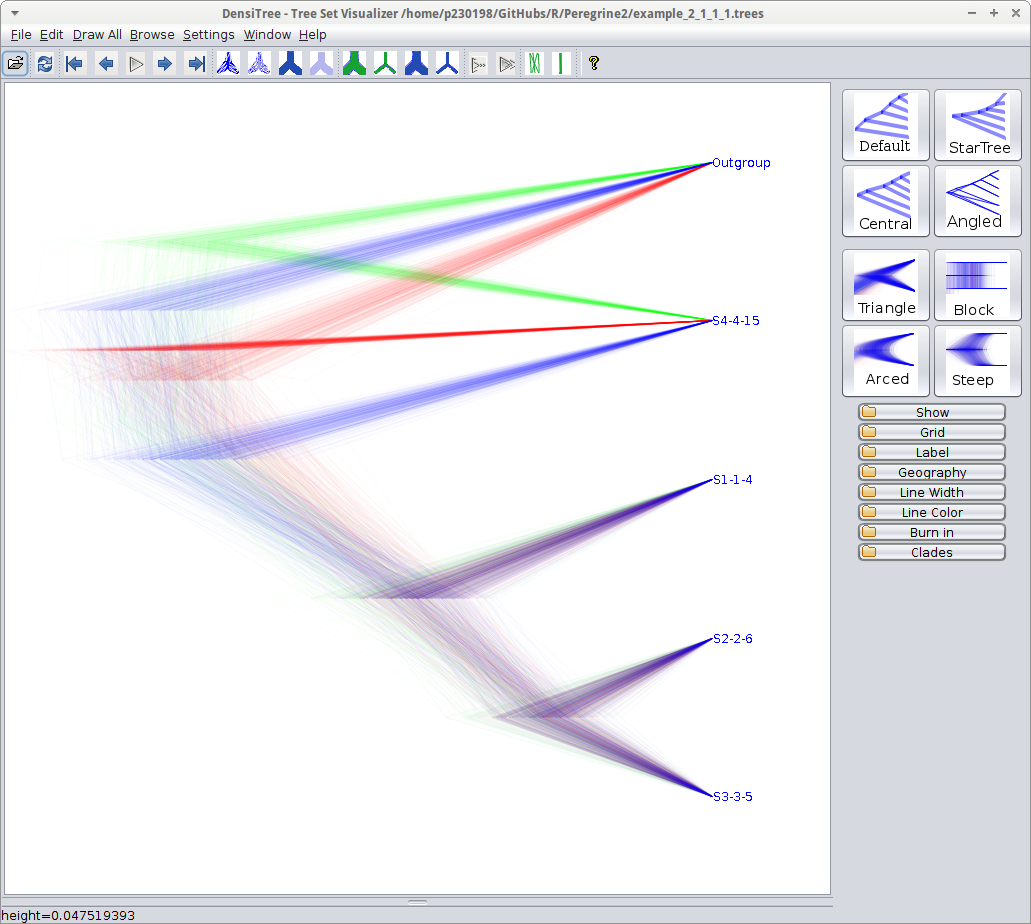
\includegraphics[width=0.5\textwidth]{example_2_densitree}

\caption{Example 2 its posterior its phylogenies\label{fig:Example-2-densitree}}
\end{figure}


When scoring the nLTT statistic between the true species tree to every
tree in the posterior, this will results in the histogram as shown
in figure \ref{fig:Example-2-nltt-stats}:

\begin{figure}[H]
\includegraphics[width=0.5\textwidth]{/home/p230198/GitHubs/R/Peregrine/example_2_nltt_stats_1_1_1}

\caption{Histogram of the nLTT statistic between the true species tree and
the trees in the posterior\label{fig:Example-2-nltt-stats}}
\end{figure}


This histogram looks a bit like a Gamma distribution, with a median
at $0.75$-$0.80$ {[}?TODO: test if this is so?{]}. 

But this does not tell us where the errors have been made: near the
crown, near the tips, or in between? To do so, we plot the average
nLTT plot of the posterior and compare it to the true species tree
its nLTT, as shown in figure \ref{fig:Example-2-posterior-average-nltt}:

\begin{figure}[H]
\includegraphics[width=0.5\textwidth]{/home/p230198/GitHubs/R/Peregrine/example_2_posterior_average_nltt_1_1_1}

\caption{Average nLTT of all the trees in the posterior. Full line: nLTT of
true species tree. Dotted line: average nLTT of all posterior trees\label{fig:Example-2-posterior-average-nltt}}
\end{figure}


Here we can see that the posterior builds up its branches around certain
timepoints: suitable phylogenies obtain their first added branch between
0.0-0.3, their second between 0.3 and 0.6, and their third between
0.6 and 0.9. This nearly always lags the true species tree.


\subsection{Comparing example 1 and 2\label{sub:Comparing-example-1-and-2}}

Both examples showed a histogram of the error between true species
tree and posterior trees. We expect these errors to have a different
distribution: example \#1 assumed instant speciation, which suits
the algorithm best, where example \#2 has a strong protractedness.
Plotting both histograms in the same plot results in figure \ref{fig:Example-both-nltt-stats}:

\begin{figure}[H]
\includegraphics[width=0.5\textwidth]{/home/p230198/GitHubs/R/Peregrine/example_12_nltt_stats_histogram}

\caption{Histogram of the nLTT statistic of the two examples \label{fig:Example-both-nltt-stats}}
\end{figure}


It can be observed that these error distributions have a different
median. This means that there is an observable higher error being
made when the true species tree is protracted. 

This visualization does not tell use how the error is made: is the
error concentrated at the root, middle or tips of the tree? To locate
this, the average nLTT plots of the posterior is shown in figure :

\begin{figure}[H]
\includegraphics[width=0.5\textwidth]{/home/p230198/GitHubs/R/Peregrine/example_12_average_nltts}

\caption{Average nLTTs of the posteriors of example \#1 (weak protractedness,
solid line) and example \#2 (strong protractedness, dotted line)\label{fig:Examples-posterior-average-nltt}}
\end{figure}



\subsection{Example 3: Weak protractedness with replicates}

This example is an extension of the examples 1, with the differences
that:
\begin{itemize}
\item From the (same) gene tree, multiple species trees are sampled
\item Per species tree, multiple DNA alignments are simulated
\item Per DNA alignment, multiple BEAST2 runs are performed
\end{itemize}

\subsubsection{Gene tree}

The first step is to simulate a gene tree. Because the RNG seed is
at the same value as example \#1, exactly the same gene tree will
be obtained, as can be seen in figure \ref{fig:Example-3-gene-tree}:

\begin{figure}[H]
\includegraphics[width=0.5\textwidth]{/home/p230198/GitHubs/R/Peregrine/example_3_gene_tree}

\caption{Example 3 gene tree. The taxon labels are S{[}genus{]}-{[}species{]}-{[}sub-species{]}'\label{fig:Example-3-gene-tree}}
\end{figure}



\subsubsection{Species tree}

It has little use to sample multiple species trees from a gene tree,
as these are identical for instant speciation models. In this example,
we do sample a species trees twice from the true gene tree. This results
in two identical species trees, as can be verified by figure \ref{fig:Example-3-species-tree}:

\begin{figure}[H]
\includegraphics[width=0.5\textwidth]{/home/p230198/GitHubs/R/Peregrine/example_3_species_tree_with_outgroup_1}\includegraphics[width=0.5\textwidth]{/home/p230198/GitHubs/R/Peregrine/example_3_species_tree_with_outgroup_nltt_1}

\includegraphics[width=0.5\textwidth]{/home/p230198/GitHubs/R/Peregrine/example_3_species_tree_with_outgroup_2}\includegraphics[width=0.5\textwidth]{/home/p230198/GitHubs/R/Peregrine/example_3_species_tree_with_outgroup_nltt_2}

\caption{Example 3 species tree and nLTT plot of that species tree\label{fig:Example-3-species-tree}}
\end{figure}



\subsubsection{Alignment}

From these (in this case identical) species trees, multiple alignments
can be simulated. In this example, for every species tree, there are
two alignments simulated. Because in this example, there are two species
sampled, and every species tree has two alignments simulated, this
results in four alignments.

Figure \ref{fig:Example-3-alignment} shows a visualisation of the
simulated alignments of our example:

\begin{figure}
\includegraphics[width=0.5\textwidth]{/home/p230198/GitHubs/R/Peregrine/example_3_alignment_1_1}\includegraphics[width=0.5\textwidth]{/home/p230198/GitHubs/R/Peregrine/example_3_alignment_1_2}

\includegraphics[width=0.5\textwidth]{/home/p230198/GitHubs/R/Peregrine/example_3_alignment_2_1}\includegraphics[width=0.5\textwidth]{/home/p230198/GitHubs/R/Peregrine/example_3_alignment_2_2}

\caption{Example 3 alignments\label{fig:Example-3-alignment}}
\end{figure}


Each alignment is different.


\subsubsection{Posterior}

In this example, for each alignment, we do two BEAST2 runs, instead
of one. It is expected (or: it should be the case) that both runs
create a similar posterior. Because this example has 2 species trees,
2 alignments per species tree and 2 BEAST2 runs per alignment, 8 different-yet-similar
posteriors are expected.

The last trees picked from the eight different posterior are shown
in figure \ref{fig:Example-3-posterior-sample-tree}:

\begin{figure}
\includegraphics[width=0.35\textwidth]{/home/p230198/GitHubs/R/Peregrine/example_3_posterior_sample_1_1_1}\includegraphics[width=0.35\textwidth]{/home/p230198/GitHubs/R/Peregrine/example_3_posterior_sample_1_1_2}

\includegraphics[width=0.35\textwidth]{/home/p230198/GitHubs/R/Peregrine/example_3_posterior_sample_1_2_1}\includegraphics[width=0.35\textwidth]{/home/p230198/GitHubs/R/Peregrine/example_3_posterior_sample_1_2_2}

\includegraphics[width=0.35\textwidth]{/home/p230198/GitHubs/R/Peregrine/example_3_posterior_sample_2_1_1}\includegraphics[width=0.35\textwidth]{/home/p230198/GitHubs/R/Peregrine/example_3_posterior_sample_2_1_2}

\includegraphics[width=0.35\textwidth]{/home/p230198/GitHubs/R/Peregrine/example_3_posterior_sample_2_2_1}\includegraphics[width=0.35\textwidth]{/home/p230198/GitHubs/R/Peregrine/example_3_posterior_sample_2_2_2}

\caption{The random species trees from example 3 its posteriors\label{fig:Example-3-posterior-sample-tree}}
\end{figure}


The species tree picked from the posterior all are different, but
not too different (figure \ref{fig:Example-3-species-tree}). Each
its nLTT plot is compared to the original species tree, which is shown
in figure \ref{fig:Example-3-both-nLTTs}:

\begin{figure}
\includegraphics[width=0.35\textwidth]{/home/p230198/GitHubs/R/Peregrine/example_3_posterior_sample_nltt_1_1_1}\includegraphics[width=0.35\textwidth]{/home/p230198/GitHubs/R/Peregrine/example_3_posterior_sample_nltt_1_1_2}

\includegraphics[width=0.35\textwidth]{/home/p230198/GitHubs/R/Peregrine/example_3_posterior_sample_nltt_1_2_1}\includegraphics[width=0.35\textwidth]{/home/p230198/GitHubs/R/Peregrine/example_3_posterior_sample_nltt_1_2_2}

\includegraphics[width=0.35\textwidth]{/home/p230198/GitHubs/R/Peregrine/example_3_posterior_sample_nltt_2_1_1}\includegraphics[width=0.35\textwidth]{/home/p230198/GitHubs/R/Peregrine/example_3_posterior_sample_nltt_2_1_2}

\includegraphics[width=0.35\textwidth]{/home/p230198/GitHubs/R/Peregrine/example_3_posterior_sample_nltt_2_2_1}\includegraphics[width=0.35\textwidth]{/home/p230198/GitHubs/R/Peregrine/example_3_posterior_sample_nltt_2_2_2}

\caption{All example 3 its nLTT plots compare to the true species tree nLTT.
The solid black line is the 'true' or initial (species) tree (with
outgroup), the dotted line is one of the trees in the BEAST2 posterioir\label{fig:Example-3-both-nLTTs}}
\end{figure}


In all cases, we can observe that the lines are close, but do not
match. Also this is expected, due to stochasticity in the MCMC sampling.

For each tree in each of the posteriors, the error is put in a histogram
as shown by figure \ref{fig:Example-3-nltt-stats}:

\begin{figure}
\includegraphics[width=0.35\textwidth]{/home/p230198/GitHubs/R/Peregrine/example_3_nltt_stats_1_1_1}\includegraphics[width=0.35\textwidth]{/home/p230198/GitHubs/R/Peregrine/example_3_nltt_stats_1_1_2}

\includegraphics[width=0.35\textwidth]{/home/p230198/GitHubs/R/Peregrine/example_3_nltt_stats_1_2_1}\includegraphics[width=0.35\textwidth]{/home/p230198/GitHubs/R/Peregrine/example_3_nltt_stats_1_2_2}

\includegraphics[width=0.35\textwidth]{/home/p230198/GitHubs/R/Peregrine/example_3_nltt_stats_2_1_1}\includegraphics[width=0.35\textwidth]{/home/p230198/GitHubs/R/Peregrine/example_3_nltt_stats_2_1_2}

\includegraphics[width=0.35\textwidth]{/home/p230198/GitHubs/R/Peregrine/example_3_nltt_stats_2_2_1}\includegraphics[width=0.35\textwidth]{/home/p230198/GitHubs/R/Peregrine/example_3_nltt_stats_2_2_2}

\caption{Histogram of the nLTT statistic between the true species tree and
the trees in the posterior\label{fig:Example-3-nltt-stats}}
\end{figure}


But this does not tell us where the errors have been made: near the
crown, near the tips, or in between? To do so, we plot the average
nLTT plot of the posterior and compare it to the true species tree
its nLTT, as shown in figure \ref{fig:Example-3-posterior-average-nltt}:

\begin{figure}
\includegraphics[width=0.35\textwidth]{/home/p230198/GitHubs/R/Peregrine/example_3_posterior_average_nltt_1_1_1}\includegraphics[width=0.35\textwidth]{/home/p230198/GitHubs/R/Peregrine/example_3_posterior_average_nltt_1_1_2}

\includegraphics[width=0.35\textwidth]{/home/p230198/GitHubs/R/Peregrine/example_3_posterior_average_nltt_1_2_1}\includegraphics[width=0.35\textwidth]{/home/p230198/GitHubs/R/Peregrine/example_3_posterior_average_nltt_1_2_2}

\includegraphics[width=0.35\textwidth]{/home/p230198/GitHubs/R/Peregrine/example_3_posterior_average_nltt_2_1_1}\includegraphics[width=0.35\textwidth]{/home/p230198/GitHubs/R/Peregrine/example_3_posterior_average_nltt_2_1_2}

\includegraphics[width=0.35\textwidth]{/home/p230198/GitHubs/R/Peregrine/example_3_posterior_average_nltt_2_2_1}\includegraphics[width=0.35\textwidth]{/home/p230198/GitHubs/R/Peregrine/example_3_posterior_average_nltt_2_2_2}

\caption{Average nLTT of all the trees in the posterior. Solid line: nLTT of
true species tree. Dotted line: average nLTT of all posterior trees\label{fig:Example-3-posterior-average-nltt}}
\end{figure}



\subsection{Example 4: Strong protractedness with replicates}

This example is an extension of the previous examples, with the differences
that:
\begin{itemize}
\item From the (same) gene tree, multiple species trees are sampled
\item Per species tree, multiple DNA alignments are simulated
\item Per DNA alignment, multiple BEAST2 runs are performed
\end{itemize}

\subsubsection{Gene tree}

The first step is to simulate a gene tree. Because the RNG seed is
at the same value as example \#1, exactly the same gene tree will
be obtained, as can be seen in figure \ref{fig:Example-4-gene-tree}:

\begin{figure}[H]
\includegraphics[width=0.5\textwidth]{/home/p230198/GitHubs/R/Peregrine/example_4_gene_tree}

\caption{Example 4 gene tree. The taxon labels are S{[}genus{]}-{[}species{]}-{[}sub-species{]}'\label{fig:Example-4-gene-tree}}
\end{figure}



\subsubsection{Species tree}

As there are multiple sub-species present for the same species, it
makes sense to sample multiple species trees from a gene tree. In
this example, we do sample a species trees twice from the true gene
tree. This results in two different species trees, as can be verified
by figure \ref{fig:Example-4-species-tree}.

\begin{figure}
\includegraphics[width=0.5\textwidth]{/home/p230198/GitHubs/R/Peregrine/example_4_species_tree_with_outgroup_1}\includegraphics[width=0.5\textwidth]{/home/p230198/GitHubs/R/Peregrine/example_4_species_tree_with_outgroup_nltt_1}

\includegraphics[width=0.5\textwidth]{/home/p230198/GitHubs/R/Peregrine/example_4_species_tree_with_outgroup_2}\includegraphics[width=0.5\textwidth]{/home/p230198/GitHubs/R/Peregrine/example_4_species_tree_with_outgroup_nltt_2}

\caption{Example 4 species tree and nLTT plot of that species tree\label{fig:Example-4-species-tree}}
\end{figure}


It is a bit of bad luck that the random number generator picked two
very similar species trees: would, instead of 


\subsubsection{Alignment}

From these (in this case identical) species trees, multiple alignments
can be simulated. In this example, for every species tree, there are
two alignments simulated. Because in this example, there are two species
sampled, and every species tree has two alignments simulated, this
results in four alignments.

Figure \ref{fig:Example-4-alignments} shows a visualisation of the
simulated alignments of our example.

\begin{figure}
\includegraphics[width=0.5\textwidth]{/home/p230198/GitHubs/R/Peregrine/example_4_alignment_1_1}\includegraphics[width=0.5\textwidth]{/home/p230198/GitHubs/R/Peregrine/example_4_alignment_1_2}

\includegraphics[width=0.5\textwidth]{/home/p230198/GitHubs/R/Peregrine/example_4_alignment_2_1}\includegraphics[width=0.5\textwidth]{/home/p230198/GitHubs/R/Peregrine/example_4_alignment_2_2}

\caption{Example 4 alignments\label{fig:Example-4-alignments}}
\end{figure}


Each alignment is different.


\subsubsection{Posterior}

In this example, for each alignment, we do two BEAST2 runs, instead
of one. It is expected (or: it should be the case) that both runs
create a similar posterior. Because this example has 2 species trees,
2 alignments per species tree and 2 BEAST2 runs per alignment, 8 different-yet-similar
posteriors are expected.

The last trees picked from the eight different posterior are shown
in figure \ref{fig:Example-4-posterior-sample-tree}.

\begin{figure}
\includegraphics[width=0.35\textwidth]{/home/p230198/GitHubs/R/Peregrine/example_4_posterior_sample_1_1_1}\includegraphics[width=0.35\textwidth]{/home/p230198/GitHubs/R/Peregrine/example_4_posterior_sample_1_1_2}

\includegraphics[width=0.35\textwidth]{/home/p230198/GitHubs/R/Peregrine/example_4_posterior_sample_1_2_1}\includegraphics[width=0.35\textwidth]{/home/p230198/GitHubs/R/Peregrine/example_4_posterior_sample_1_2_2}

\includegraphics[width=0.35\textwidth]{/home/p230198/GitHubs/R/Peregrine/example_4_posterior_sample_2_1_1}\includegraphics[width=0.35\textwidth]{/home/p230198/GitHubs/R/Peregrine/example_4_posterior_sample_2_1_2}

\includegraphics[width=0.35\textwidth]{/home/p230198/GitHubs/R/Peregrine/example_4_posterior_sample_2_2_1}\includegraphics[width=0.35\textwidth]{/home/p230198/GitHubs/R/Peregrine/example_4_posterior_sample_2_2_2}

\caption{The random species trees from example 3 its posteriors\label{fig:Example-4-posterior-sample-tree}}
\end{figure}


The species tree picked from the posterior all are different, but
not too different (figure \ref{fig:Example-4-species-tree}). Each
its nLTT plot is compared to the original species tree, which is shown
in figure \ref{fig:Example-4-both-nLTTs}.

\begin{figure}
\includegraphics[width=0.35\textwidth]{/home/p230198/GitHubs/R/Peregrine/example_4_posterior_sample_nltt_1_1_1}\includegraphics[width=0.35\textwidth]{/home/p230198/GitHubs/R/Peregrine/example_4_posterior_sample_nltt_1_1_2}

\includegraphics[width=0.35\textwidth]{/home/p230198/GitHubs/R/Peregrine/example_4_posterior_sample_nltt_1_2_1}\includegraphics[width=0.35\textwidth]{/home/p230198/GitHubs/R/Peregrine/example_4_posterior_sample_nltt_1_2_2}

\includegraphics[width=0.35\textwidth]{/home/p230198/GitHubs/R/Peregrine/example_4_posterior_sample_nltt_2_1_1}\includegraphics[width=0.35\textwidth]{/home/p230198/GitHubs/R/Peregrine/example_4_posterior_sample_nltt_2_1_2}

\includegraphics[width=0.35\textwidth]{/home/p230198/GitHubs/R/Peregrine/example_4_posterior_sample_nltt_2_2_1}\includegraphics[width=0.35\textwidth]{/home/p230198/GitHubs/R/Peregrine/example_4_posterior_sample_nltt_2_2_2}

\caption{All example 4 its nLTT plots compare to the true species tree nLTT.
The solid black line is the 'true' or initial (species) tree (with
outgroup), the dotted line is one of the trees in the BEAST2 posterioir\label{fig:Example-4-both-nLTTs}}
\end{figure}


In all cases, we can observe that the lines are close, but do not
match. Also this is expected, due to stochasticity in the MCMC sampling.

For each tree in each of the posteriors, the error is put in a histogram
as shown by figure \ref{fig:Example-4-nltt-stats}.

\begin{figure}
\includegraphics[width=0.35\textwidth]{/home/p230198/GitHubs/R/Peregrine/example_4_nltt_stats_1_1_1}\includegraphics[width=0.35\textwidth]{/home/p230198/GitHubs/R/Peregrine/example_4_nltt_stats_1_1_2}

\includegraphics[width=0.35\textwidth]{/home/p230198/GitHubs/R/Peregrine/example_4_nltt_stats_1_2_1}\includegraphics[width=0.35\textwidth]{/home/p230198/GitHubs/R/Peregrine/example_4_nltt_stats_1_2_2}

\includegraphics[width=0.35\textwidth]{/home/p230198/GitHubs/R/Peregrine/example_4_nltt_stats_2_1_1}\includegraphics[width=0.35\textwidth]{/home/p230198/GitHubs/R/Peregrine/example_4_nltt_stats_2_1_2}

\includegraphics[width=0.35\textwidth]{/home/p230198/GitHubs/R/Peregrine/example_4_nltt_stats_2_2_1}\includegraphics[width=0.35\textwidth]{/home/p230198/GitHubs/R/Peregrine/example_4_nltt_stats_2_2_2}

\caption{Histogram of the nLTT statistic between the true species tree and
the trees in the posterior\label{fig:Example-4-nltt-stats}}
\end{figure}


But this does not tell us where the errors have been made: near the
crown, near the tips, or in between? To do so, we plot the average
nLTT plot of the posterior and compare it to the true species tree
its nLTT, as shown in figure \ref{fig:Example-4-posterior-average-nltt}.

\begin{figure}
\includegraphics[width=0.35\textwidth]{/home/p230198/GitHubs/R/Peregrine/example_4_posterior_average_nltt_1_1_1}\includegraphics[width=0.35\textwidth]{/home/p230198/GitHubs/R/Peregrine/example_4_posterior_average_nltt_1_1_2}

\includegraphics[width=0.35\textwidth]{/home/p230198/GitHubs/R/Peregrine/example_4_posterior_average_nltt_1_2_1}\includegraphics[width=0.35\textwidth]{/home/p230198/GitHubs/R/Peregrine/example_4_posterior_average_nltt_1_2_2}

\includegraphics[width=0.35\textwidth]{/home/p230198/GitHubs/R/Peregrine/example_4_posterior_average_nltt_2_1_1}\includegraphics[width=0.35\textwidth]{/home/p230198/GitHubs/R/Peregrine/example_4_posterior_average_nltt_2_1_2}

\includegraphics[width=0.35\textwidth]{/home/p230198/GitHubs/R/Peregrine/example_4_posterior_average_nltt_2_2_1}\includegraphics[width=0.35\textwidth]{/home/p230198/GitHubs/R/Peregrine/example_4_posterior_average_nltt_2_2_2}

\caption{Average nLTT of all the trees in the posterior. Solid line: nLTT of
true species tree. Dotted line: average nLTT of all posterior trees\label{fig:Example-4-posterior-average-nltt}}
\end{figure}



\subsection{Comparing example 3 and 4}

Both examples showed a histogram of the error between true species
tree and posterior trees. We expect these errors to have a different
distribution: example \#1 assumed instant speciation, which suits
the algorithm best, where example \#2 has a strong protractedness.
Plotting both histograms in the same plot results in figure \ref{fig:Example-34-both-nltt-stats}:

\begin{figure}[H]
\includegraphics[width=0.5\textwidth]{/home/p230198/GitHubs/R/Peregrine/example_34_nltt_stats_histogram}

\caption{Histogram of the nLTT statistic of the two examples \label{fig:Example-34-both-nltt-stats}}
\end{figure}


It can be observed that these error distributions have a different
median. This means that there is an observable higher error being
made when the true species tree is protracted. 

This visualization does not tell use how the error is made: is the
error concentrated at the root, middle or tips of the tree? To locate
this, the average nLTT plots of the posterior is shown in figure \ref{fig:Examples-34-posterior-average-nltt}:

\begin{figure}[H]
\includegraphics[width=0.5\textwidth]{/home/p230198/GitHubs/R/Peregrine/example_34_average_nltts}

\caption{Average nLTTs of the posteriors of example \#3 (weak protractedness,
solid line) and example \#4 (strong protractedness, dotted line)\label{fig:Examples-34-posterior-average-nltt}}
\end{figure}



\section{Bash scripts}

Files that are called from the command line.


\subsection{check\_example\_parameter\_files.sh\label{sub:check_example_parameter_files.sh}}

This bash script shows how to check the example parameter files:

\begin{algorithm}[H]
\lstinputlisting[breaklines=true,language=bash,showstringspaces=false]{/home/p230198/GitHubs/R/Peregrine/check_example_parameter_files.sh}

\caption{The 'check\_example\_parameter\_files.sh' script \label{alg:check_example_parameter_files.sh}}
\end{algorithm}


The bash script indicates in its first line that it is a bash script.
The next two lines call an R script file called 'check\_parameter\_file.R'
(see chapter \ref{sub:check_parameter_file.R}) with the parameter
filename.

\begin{algorithm}[H]
\verbatiminput{/home/p230198/GitHubs/R/Peregrine2/check_example_parameter_files.txt}

\caption{Output of 'check\_example\_parameter\_files.sh' \label{alg:check_example_parameter_files.txt}}
\end{algorithm}



\subsection{create\_article\_parameter\_files.sh\label{sub:create_article_parameter_files.sh}}

\begin{algorithm}[H]
\lstinputlisting[breaklines=true,language=bash,showstringspaces=false]{/home/p230198/GitHubs/R/Peregrine/create_article_parameter_files.sh}

\caption{The 'create\_article\_parameter\_files.sh' script \label{alg:create_article_parameter_file.sh}}
\end{algorithm}


The first line indicates that this file is a bash script. Then it
creates all parameter files.


\subsection{create\_article\_parameter\_files\_job.sh\label{sub:create_article_parameter_files_job.sh}}

\begin{algorithm}[H]
\lstinputlisting[breaklines=true,language=bash,showstringspaces=false]{/home/p230198/GitHubs/R/Peregrine/create_article_parameter_files_job.sh}

\caption{The 'create\_article\_parameter\_files\_job.sh' script \label{alg:create_article_parameter_file.sh-1}}
\end{algorithm}


A Peregrine cluster job script, calling 'create\_article\_parameter\_files.sh'
(chapter \ref{sub:create_article_parameter_files.sh}).

On the Peregrine cluster, call this with:

\begin{lstlisting}
sbatch ./create_article_parameter_files_job.sh
\end{lstlisting}



\subsection{create\_example\_parameter\_files.sh\label{sub:create_example_parameter_file.sh}}

\begin{algorithm}[H]
\lstinputlisting[breaklines=true,language=bash,showstringspaces=false]{/home/p230198/GitHubs/R/Peregrine/create_example_parameter_files.sh}

\caption{The 'create\_example\_parameter\_files.sh' script \label{alg:create_example_parameter_file.sh}}
\end{algorithm}


The first line indicates that this file is a bash script. The next
two lines call the R script file called 'create\_parameter\_file.R'
(see chapter TODO) with the 14 parameter arguments.


\subsection{do\_analyze\_examples.sh}

This bash script analyzes the the results of the worked-out examples
(chapter \ref{sec:Worked-out-examples}) and is displayed in algorithm
\ref{alg:do_analyze_examples.sh}:

\begin{algorithm}[H]
\lstinputlisting[breaklines=true,language=bash,showstringspaces=false]{/home/p230198/GitHubs/R/Peregrine/do_analyze_examples.sh}

\caption{The 'do\_analyze\_examples.sh' script \label{alg:do_analyze_examples.sh}}
\end{algorithm}


The first line of the file indicates that it is a bash script. Then
the R script file 'do\_analyze.R' (see chapter \ref{sub:do_analyze.R})
is called with one or more parameter filenames.


\subsection{do\_simulation\_examples.sh\label{sub:do_simulation_examples.sh}}

This scripts runs all simulations of the worked-out examples, as shown
in algorithm \ref{alg:do_simulation_examples.sh}:

\begin{algorithm}[H]
\lstinputlisting[breaklines=true,language=bash,showstringspaces=false]{/home/p230198/GitHubs/R/Peregrine/do_simulation_examples.sh}

\caption{The 'do\_simulation\_examples.sh' script \label{alg:do_simulation_examples.sh}}
\end{algorithm}


The bash script indicates in its first line that it is a bash script,
then call an R script file called 'do\_simulation.R' (see chapter
\ref{sub:do_simulation.R}) with the parameter file its name. 


\subsection{sbatch\_all.sh\label{sub:sbatch_all.sh}}

This scripts submits all jobs to the computercluster, as shown in
algorithm \ref{alg:sbatch_all.sh}:

\begin{algorithm}[H]
\lstinputlisting[breaklines=true,language=bash,showstringspaces=false]{/home/p230198/GitHubs/R/Peregrine/sbatch_all.sh}

\caption{The 'sbatch\_all.sh' script \label{alg:sbatch_all.sh}}
\end{algorithm}


The bash script indicates in its first line that it is a bash script.
Then, for every file with an .RDa extension, sbatch the 'sbatch\_me.sh'
(see chapter \ref{sub:do_simulation.R}) with the parameter file its
name. 


\subsection{sbatch\_me.sh\label{sub:sbatch_me.sh}}

This scripts runs a simulation on a computer cluster. It is shown
in algorithm \ref{alg:sbatch_me.sh}:

\begin{algorithm}[H]
\lstinputlisting[breaklines=true,language=bash,showstringspaces=false]{/home/p230198/GitHubs/R/Peregrine/sbatch_me.sh}

\caption{The 'sbatch\_me.sh' script \label{alg:sbatch_me.sh}}
\end{algorithm}


The bash script indicates in its first line that it is a bash script.
Then it sets up the computer cluster parameters, loads the modules
for BEAST2 and R, then runs a simulation for the parameter filename
given as its first argument when called.


\section{R scripts}

Files that are run standalone and can be called from the command line.


\subsection{check\_parameter\_file.R\label{sub:check_parameter_file.R}}

The R script 'check\_parameter\_file.R' file prints out the parameters
and its code is shown in algorithm \ref{alg:check_parameter_file.R}:

\begin{algorithm}[H]
\lstinputlisting[breaklines=true,language=R,showstringspaces=false]{/home/p230198/GitHubs/R/Peregrine/check_parameter_file.R}

\caption{The 'check\_parameter\_file.R' script \label{alg:check_parameter_file.R}}
\end{algorithm}


First, 'check\_parameter\_file.R' checks if the parameter exists,
after which it displays the parameter values. 

The bash script 'check\_example\_parameter\_files.sh' (see chapter
\ref{sub:check_example_parameter_files.sh}) shows how to the example
parameter files are checked.


\subsection{create\_parameter\_file.R\label{sub:create_parameter_file.R}}

\begin{algorithm}[H]
\lstinputlisting[breaklines=true,language=R,showstringspaces=false]{/home/p230198/GitHubs/R/Peregrine/create_parameter_file.R}

\caption{The 'create\_parameter\_file.R' script \label{alg:create_parameter_file.R}}
\end{algorithm}


Creates a parameter file from the parameters supplied. First, 'create\_parameter\_file.R'
checks if there are the right amount of parameters, with the correct
form. The last argument is the parameter file its filename. As the
parameter file uses the R data format, it is fitting to use the '.RDa'
extension.

Most of the work is then pushed forward to the 'save\_parameters\_to\_file'
function, which is described in chapter \ref{sub:save_parameters_to_file}.

The bash script 'create\_example\_parameter\_files.sh' (see chapter
\ref{sub:create_example_parameter_file.sh}) shows how to create the
example parameter files.


\subsection{do\_analyze.R\label{sub:do_analyze.R}}

Performs the analysis and creates the result graphs, as shown in algorithm
\ref{alg:do_analyze.R}:

\begin{algorithm}
\lstinputlisting[breaklines=true,language=R,showstringspaces=false]{/home/p230198/GitHubs/R/Peregrine/do_analyze.R}

\caption{The 'do\_analyze.R' script \label{alg:do_analyze.R}}
\end{algorithm}


This script it behavior depends on the number of arguments supplied
from the command line:
\begin{itemize}
\item one parameter filename: create the graphs of a single run using the
R function 'do\_analyze\_single' (see chapter \ref{sub:do_analyze_single})
\item multiple parameter filenames: create the graphs of mutiple runs using
the R function 'do\_analyze\_multi' (see chapter \ref{sub:do_analyze_multi})
\end{itemize}

\subsection{do\_simulation.R\label{sub:do_simulation.R}}

Performs the simulation for a parameter file, as shown in algorithm
\ref{alg:do_simulation.R}:

\begin{algorithm}[H]
\lstinputlisting[breaklines=true,language=R,showstringspaces=false]{/home/p230198/GitHubs/R/Peregrine/do_simulation.R}

\caption{The 'do\_simulation.R' script \label{alg:do_simulation.R}}
\end{algorithm}


'do\_simulation.R' first checks if the supplied function argument
is an existing filename. Then, it runs all the steps from the experiment,
by calling these functions:
\begin{itemize}
\item 'add\_pbd\_output': from the parameters, create a gene tree (see chapter
\ref{sub:add_pbd_output})
\item 'add\_species\_trees\_with\_outgroup': from the gene tree, create
one or more species trees with an added outgroup (see chapter \ref{sub:add_species_trees_with_outgroup})
\item 'add\_alignments': from each species tree (with outgroup), create
one or more simulated DNA alignments (see chapter \ref{sub:add_alignments})
\item 'add\_posteriors': for each DNA alignment, create one or more BEAST2
posterior files (see chapter \ref{sub:add_posteriors})
\end{itemize}
The 'do\_simulation\_examples.sh' bash script (see chapter \ref{sub:do_simulation_examples.sh})
shows how to call 'do\_simulation' for the worked-out examples. 


\section{R functions}

Functions that are called.

The functions used are listed here alphabetically. The chronological
order of these function calls is shown in figure \ref{fig:Code-flow}:

\begin{figure}[H]
\includegraphics[width=0.33\textwidth]{Workflow_code}

\caption{The chronological order of the functions called\label{fig:Code-flow}}
\end{figure}



\subsection{add\_alignments\label{sub:add_alignments}}

Create a simulated DNA alignment from a species tree (with outgroup).
See algorithm \ref{alg:add_alignments.R}.

\begin{algorithm}
\lstinputlisting[breaklines=true,language=R,showstringspaces=false]{/home/p230198/GitHubs/R/Peregrine/add_alignments.R}

\caption{The 'add\_alignments' function \label{alg:add_alignments.R}}
\end{algorithm}



\subsection{add\_pbd\_output\label{sub:add_pbd_output}}

Creates a gene tree from a parameter file. See algorithm \ref{alg:add_pbd_output.R}.

\begin{algorithm}
\lstinputlisting[breaklines=true,language=R,showstringspaces=false]{/home/p230198/GitHubs/R/Peregrine/add_pbd_output.R}

\caption{The 'add\_pbd\_output' function \label{alg:add_pbd_output.R}}
\end{algorithm}



\subsection{add\_posteriors\label{sub:add_posteriors}}

For each DNA alignment, create one or more BEAST2 posterior files.
See algorithm \ref{alg:add_posteriors.R}.

\begin{algorithm}
\lstinputlisting[breaklines=true,language=R,showstringspaces=false]{/home/p230198/GitHubs/R/Peregrine/add_posteriors.R}

\caption{The 'add\_posteriors' function \label{alg:add_posteriors.R}}
\end{algorithm}



\subsection{add\_species\_trees\_with\_outgroup\label{sub:add_species_trees_with_outgroup}}

Creates one or more species trees from a gene tree. Also adds an outgroup
to each species tree. See algorithm \ref{alg:add_species_trees_with_outgroup.R}.

\begin{algorithm}
\lstinputlisting[breaklines=true,language=R,showstringspaces=false]{/home/p230198/GitHubs/R/Peregrine/add_species_trees_with_outgroup.R}

\caption{The 'add\_species\_trees\_with\_outgroup' function \label{alg:add_species_trees_with_outgroup.R}}
\end{algorithm}



\subsection{do\_analyze\_multi\label{sub:do_analyze_multi}}

R function that is called to creates the result graphs for a multiple
parameter filenames. This is useful to do comparisons: the first filename
is assumed to be a non-protracted parameter file. See algorithm \ref{alg:do_analyze_multi.R}.

\begin{algorithm}
\lstinputlisting[breaklines=true,language=R,showstringspaces=false]{/home/p230198/GitHubs/R/Peregrine/do_analyze_multi.R}

\caption{The 'do\_analyze\_multi' function \label{alg:do_analyze_multi.R}}
\end{algorithm}


It forwards the heavy lifting to other R functions.


\subsection{do\_analyze\_single\label{sub:do_analyze_single}}

R function that is called to creates the result graphs for a single
parameter filename. See algorithm \ref{alg:do_analyze_single.R}.

\begin{algorithm}
\lstinputlisting[breaklines=true,language=R,showstringspaces=false]{/home/p230198/GitHubs/R/Peregrine/do_analyze_single.R}

\caption{The 'do\_analyze\_single' function \label{alg:do_analyze_single.R}}
\end{algorithm}


It forwards the heavy lifting to other R functions.


\subsection{is\_valid\_file\label{sub:is_valid_file}}

The function 'is\_valid\_file' checks if a parameter file is valid,
as can be seen in algorithm \ref{alg:is_valid_file}.

\begin{algorithm}
\lstinputlisting[breaklines=true,language=R,showstringspaces=false]{/home/p230198/GitHubs/R/Peregrine/is_valid_file.R}

\caption{The 'is\_valid\_file' function \label{alg:is_valid_file}}
\end{algorithm}


It checks the parameter file its form and its parameter values.


\subsection{plot\_alignments}

This R function plots the alignments of a parameter file.

\begin{algorithm}
\lstinputlisting[breaklines=true,language=R,showstringspaces=false]{/home/p230198/GitHubs/R/Peregrine/plot_alignments.R}

\caption{The 'plot\_alignments' function \label{alg:plot_alignments}}
\end{algorithm}


Figure \ref{fig:Example-1-alignment} is produced by this function.


\subsection{plot\_gene\_tree}

This R function plots the gene tree of a parameter file.

\begin{algorithm}
\lstinputlisting[breaklines=true,language=R,showstringspaces=false]{/home/p230198/GitHubs/R/Peregrine/plot_gene_tree.R}

\caption{The 'plot\_gene\_tree' function \label{alg:plot_gene_tree}}
\end{algorithm}


There is always exactly one gene tree per parameter file. 

Figure \ref{fig:Example-1-gene-tree} is produced by this function.


\subsection{plot\_multi\_average\_nltts}

This R function plots the alignments of a parameter file.

\begin{algorithm}
\lstinputlisting[breaklines=true,language=R,showstringspaces=false]{/home/p230198/GitHubs/R/Peregrine/plot_multi_average_nltts.R}

\caption{The 'plot\_multi\_average\_nltts' function \label{alg:plot_multi_average_nltts}}
\end{algorithm}


Figure \ref{fig:Examples-posterior-average-nltt} is produced by this
function.


\subsection{plot\_multi\_nltt\_stats\_histogram}

This R function plots the alignments of a parameter file.

\begin{algorithm}
\lstinputlisting[breaklines=true,language=R,showstringspaces=false]{/home/p230198/GitHubs/R/Peregrine/plot_multi_nltt_stats_histogram.R}

\caption{The 'plot\_multi\_nltt\_stats\_histogram' function \label{alg:plot_multi_nltt_stats_histogram}}
\end{algorithm}


Figure \ref{fig:Example-both-nltt-stats} is produced by this function.


\subsection{plot\_posterior\_average\_nltts}

For each posterior, plots the average nLTT of all phylogenies, including
the true tree its nLTT.

\begin{algorithm}
\lstinputlisting[breaklines=true,language=R,showstringspaces=false]{/home/p230198/GitHubs/R/Peregrine/plot_posterior_average_nltts.R}

\caption{The 'plot\_posterior\_average\_nltts' function \label{alg:plot_posterior_average_nltts}}
\end{algorithm}


Figure \ref{fig:Example-1-posterior-average-nltt} is produced by
this function.


\subsection{plot\_posterior\_nltt\_stats\_histogram}

R function that creates a histogram out of the nLTT stats and puts
it in a histogram.

\begin{algorithm}
\lstinputlisting[breaklines=true,language=R,showstringspaces=false]{/home/p230198/GitHubs/R/Peregrine/plot_posterior_nltt_stats_histogram.R}

\caption{The 'plot\_nltt\_stats\_histogram' function \label{alg:plot_nltt_stats_histogram}}
\end{algorithm}


Figure \ref{fig:Example-1-nltt-stats} is produced by this function.


\subsection{plot\_posterior\_samples}

R function that plots a single tree in the posterior.

\begin{algorithm}
\lstinputlisting[breaklines=true,language=R,showstringspaces=false]{/home/p230198/GitHubs/R/Peregrine/plot_posterior_samples.R}

\caption{The 'plot\_posterior\_samples' function \label{alg:plot_posterior_samples}}
\end{algorithm}


Figure \ref{fig:Example-1-posterior-sample-tree} is produced by this
function.


\subsection{plot\_posterior\_sample\_nltts}

R function that plots the nLTT plot of a single tree in the posterior.

\begin{algorithm}
\lstinputlisting[breaklines=true,language=R,showstringspaces=false]{/home/p230198/GitHubs/R/Peregrine/plot_posterior_sample_nltts.R}

\caption{The 'plot\_posterior\_sample\_nltts' function \label{alg:plot_posterior_sample_nltts }}
\end{algorithm}


Figure \ref{fig:Example-1-posterior-sample-tree-nltt} is produced
by this function.


\subsection{plot\_species\_tree\_with\_outgroup}

This R function that plots the species trees of a parameter file.

\begin{algorithm}
\lstinputlisting[breaklines=true,language=R,showstringspaces=false]{/home/p230198/GitHubs/R/Peregrine/plot_species_tree_with_outgroup.R}

\caption{The 'plot\_species\_tree\_with\_outgroup' function \label{alg:plot_species_tree_with_outgroup}}
\end{algorithm}


There are $n_{species\_trees}$ species trees per parameter file,
each sampled randomly from the same species tree.

Figure \ref{fig:Example-1-species-tree} is produced by this function.


\subsection{plot\_species\_tree\_with\_outgroup\_nltt}

This R function that plots the species trees their nLTT plots of a
parameter file.

\begin{algorithm}
\lstinputlisting[breaklines=true,language=R,showstringspaces=false]{/home/p230198/GitHubs/R/Peregrine/plot_species_tree_with_outgroup_nltt.R}

\caption{The 'plot\_species\_tree\_with\_outgroup\_nltt' function \label{alg:plot_species_tree_with_outgroup_nltt}}
\end{algorithm}


There are $n_{species\_trees}$ species trees per parameter file,
each sampled randomly from the same species tree.

Figure \ref{fig:Example-1-species-tree-nltt} is produced by this
function.


\subsection{save\_parameters\_to\_file\label{sub:save_parameters_to_file}}

The function 'save\_parameters\_to\_file' saves the parameters to
file, as can be seen in algorithm \ref{alg:save_parameters_to_file.R}.

\begin{algorithm}
\lstinputlisting[breaklines=true,language=R,showstringspaces=false]{/home/p230198/GitHubs/R/Peregrine/save_parameters_to_file.R}

\caption{The 'save\_parameters\_to\_file' function \label{alg:save_parameters_to_file.R}}
\end{algorithm}


At the core of this function is the creation of 'my\_table', which
stores all the parameters. After saving, it calls 'is\_valid\_file'
to check the parameter file. Finally it checks if saving and loading
of the created parameter file works as expected.


\section{Error}


\subsection{BEAST requires Java version 8}

Sometimes my Java version degrades to version 7. BEAST2 will show
figure \ref{fig:BEAST2-error}:

\begin{figure}
\includegraphics[width=0.5\textwidth]{ErrorJava8needed}

\caption{BEAST2 error\label{fig:BEAST2-error}}


\end{figure}


On the command-line do:

\begin{lstlisting}
sudo apt-get install oracle-java8-set-default
\end{lstlisting}

\end{document}
